\documentclass[11pt,a4paper]{article}
\usepackage[utf8]{inputenc}
\usepackage{amsmath}
\usepackage{graphicx}
\usepackage[american]{circuitikz}
\usepackage{listings}
\usepackage{xcolor}
\usepackage{hyperref}
\usepackage{caption}
\usepackage{float}
\usepackage{geometry}
\geometry{margin=1in}

\begin{document}

This is the simulation of a backup power system that maintains a 5\,V, 1\,A output for 60 seconds when disconnected from power. The system utilizes 3\,V, 50\,F supercapacitors, an LM2596 buck converter, and is simulated using MATLAB. The purpose is to ensure continuous power supply during brief power outages or transitions.

\section{Circuit Diagram}

The circuit consists of four capacitors connected in series (\( C_1 \) through \( C_4 \)), a buck converter, and a load resistor (\( R_1 \)). Each capacitor is rated at 50\,F, 3\,V. The buck converter outputs a regulated 5\,V to the load resistor, which has a resistance of 5\,$\Omega$.

\begin{figure}[H]
    \centering
\begin{circuitikz}[american]
    % Draw capacitors in series
    \draw (0,0)
        to[C=$C_1$, l_=50\,F] (2,0)
        to[C=$C_2$, l_=50\,F] (4,0)
        to[C=$C_3$, l_=50\,F] (6,0)
        to[C=$C_4$, l_=50\,F] (8,0)
        to[short] (10,0); % Connection to DC-DC converter

    % DC-DC converter box
    \draw (10,-1) rectangle (12,1);
    \draw (11,0) node{LM2596};

    % Connection from capacitors to DC-DC converter
    \draw (8,0) to[short] (10,0);
    \draw (0,0) to[short] (0,-4);

    % Output from DC-DC converter to resistor R1
    \draw (12,0) to[short] (14,0)
        to[R=$R_1$, l_=5\,$\Omega$] (14,-4)
        to[short] (0,-4);

    % Ground symbols (optional)
     \draw (7,-4) node[ground]{};

    % Loop back to the start of the capacitors
    \draw (0,-4) to[short] (0,0);
\end{circuitikz}
    \caption{Circuit Diagram of the Backup Power System}
    \label{fig:circuit}
\end{figure}

\section{Simulation in MATLAB}

The system is simulated using MATLAB to model the discharge behavior of the capacitor bank through the buck converter and the load resistor. The MATLAB script utilizes the Euler method for numerical integration and switches the discharge model when the capacitor voltage drops below the buck converter's minimum operational voltage.


\lstset{language=Matlab,
        basicstyle=\ttfamily\small,
        keywordstyle=\color{blue},
        commentstyle=\color{gray},
        stringstyle=\color{red},
        numbers=left,
        numberstyle=\tiny,
        stepnumber=1,
        numbersep=5pt,
        breaklines=true,
        frame=single,
        rulecolor=\color{black},
        showstringspaces=false,
        tabsize=4,
        captionpos=b
}

\begin{lstlisting}[caption={Capacitor Discharge Simulation in MATLAB}, label={lst:matlab_code}]
% Capacitor Discharge Simulation Using Euler Method with Switching Model

% Parameters
numSeriesCaps = 4;
numParallelBranches = 1;
capVoltage = 3;
capacitance = 50;
initialCapVoltage = numSeriesCaps * capVoltage;
minBuckVoltage = 5;
totalCapacitance = (capacitance / numSeriesCaps) * numParallelBranches;
converterEfficiency = 0.9;
outputPower = 5;
inputPower = outputPower / converterEfficiency;
timeStep = 0.1;
simDuration = 300;
loadResistance = 5;

% Initialization
timeVector = 0:timeStep:simDuration;
capVoltageArray = zeros(size(timeVector));
capVoltageArray(1) = initialCapVoltage;
currentArray = zeros(size(timeVector));
buckVoltageArray = zeros(size(timeVector));

% Simulation Loop
for i = 1:length(timeVector)-1
    V = capVoltageArray(i);
    if V >= minBuckVoltage
        currentDraw = inputPower / V;
        buckVoltage = minBuckVoltage;
    else
        currentDraw = V / loadResistance;
        buckVoltage = V;
    end
    dV = -currentDraw / totalCapacitance * timeStep;
    capVoltageArray(i+1) = V + dV;
    currentArray(i) = currentDraw;
    buckVoltageArray(i) = buckVoltage;
    if capVoltageArray(i+1) <= 0
        capVoltageArray(i+1:end) = 0;
        currentArray(i+1:end) = 0;
        buckVoltageArray(i+1:end) = 0;
        disp('Capacitor voltage has reached zero.');
        break;
    end
end

if capVoltageArray(end) > 0
    currentArray(end) = currentArray(end-1);
    buckVoltageArray(end) = buckVoltageArray(end-1);
end

% Plotting
figure;
yyaxis left
plot(timeVector, capVoltageArray, 'b-', 'LineWidth', 2);
hold on;
plot(timeVector, buckVoltageArray, 'r-', 'LineWidth', 2);
ylabel('Voltage (V)');
ylim([0, max(capVoltageArray)+1]);
yyaxis right
plot(timeVector, currentArray, 'k-', 'LineWidth', 1.5);
ylabel('Current (A)');
ylim([0, max(currentArray)+1]);
xlabel('Time (s)');
title('Capacitor Voltage, Buck Converter Output, and Current Over Time');
grid on;
legend({'Capacitor Voltage', 'Buck Converter Output', 'Current Usage'}, 'Location', 'best');
hold off;
\end{lstlisting}

\subsection{Meeting the System Requirements}

\begin{figure}[h!]
    \centering
    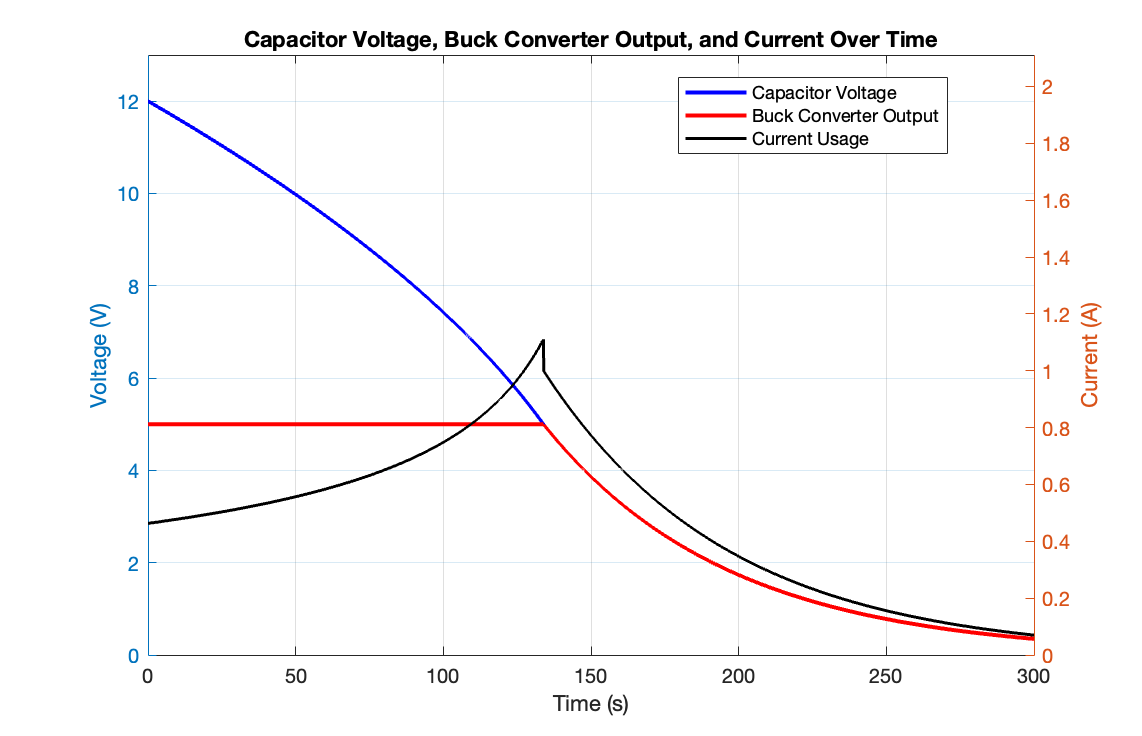
\includegraphics[width=1\textwidth]{fig.png} % Replace with actual path to the image
    \caption{Data from Super Caps}
\end{figure}

To determine if the system meets the requirement of maintaining a 5\,V, 1\,A output for 60 seconds:

\begin{itemize}
    \item \textbf{Duration of Buck Converter Operation:} Analyze the plot to find the time at which the capacitor voltage drops to 5\,V.
    \item \textbf{Energy Calculation:} The total energy stored in the capacitor bank is:
    \[
    E_{\text{stored}} = \frac{1}{2} C_{\text{total}} V_{\text{initial}}^2 = \frac{1}{2} \times 12.5\,\text{F} \times (12\,\text{V})^2 = 900\,\text{J}
    \]
    \item \textbf{Energy Required:} The energy required to maintain 5\,W output for 60 seconds is:
    \[
    E_{\text{required}} = P_{\text{out}} \times t = 5\,\text{W} \times 60\,\text{s} = 300\,\text{J}
    \]
    \item \textbf{Conclusion:} Since the stored energy exceeds the required energy, and if the buck converter operates for at least 60 seconds before the capacitor voltage drops below 5\,V, the system meets the requirements.
\end{itemize}

\section{References}

\begin{itemize}
    \item LM2596 Datasheet: \url{https://www.ti.com/lit/ds/symlink/lm2596.pdf}
\end{itemize}

\end{document}
